\documentclass[a4paper,english]{report}

\usepackage[latin1]{inputenc}
\usepackage[T1]{fontenc}
\usepackage{fourier}
\usepackage{babel,textcomp}
\usepackage[pdftex]{graphicx}
\usepackage{subfigure}
\usepackage{listings}
\usepackage{hyperref}
\usepackage{varioref}
\usepackage{cite}
\usepackage[color]{uiosloforside}
\usepackage[bottom]{footmisc}
\usepackage{tikz}
\usetikzlibrary{shapes,arrows}
\usepackage[compact]{titlesec}
\usepackage{chngcntr}
\counterwithout*{footnote}{chapter}
\setcounter{tocdepth}{1}

\setlength\topmargin{0in}
\setlength\headheight{0in}
\setlength\headsep{0in}
\setlength\textheight{9.0in}
\setlength\textwidth{6.5in}
\setlength\oddsidemargin{0in}
\setlength\evensidemargin{0in}
\setlength\parindent{0in}
\setlength\parskip{0.10in}
\setlength\columnsep{0.25in}

\definecolor{dkgreen}{rgb}{0,0.6,0}
\definecolor{gray}{rgb}{0.5,0.5,0.5}
\definecolor{lightgray}{rgb}{0.8,0.8,0.8}
\definecolor{mauve}{rgb}{0.58,0,0.82}
\definecolor{matnat}{rgb}{0.004,0.47,0.44}

% "define" Scala
\lstdefinelanguage{scala}{
  morekeywords={abstract,case,catch,class,def,
    do,else,extends,false,final,finally,
    for,if,implicit,import,match,mixin,
    new,null,object,override,package,
    private,protected,requires,return,sealed,
    super,this,throw,trait,true,try,
    type,val,var,while,with,yield},
  otherkeywords={=>,<-,<\%,<:,>:,@}, % Removed \#, because of Ruby comments error
  sensitive=true,
  morecomment=[l]{//},
  morecomment=[n]{/*}{*/},
  morestring=[b]",
  morestring=[b]',
  morestring=[b]"""
}

\lstset{basicstyle=\footnotesize,
%  columns=spaceflexible,
  numbers=none,
  numberstyle=\tiny\color{gray},
  keywordstyle=\color{blue}\bfseries,
  commentstyle=\color{dkgreen},
  stringstyle=\color{mauve},
  frame=single,
  frameround=tttt,
  rulecolor=\color{lightgray},
  showstringspaces=false,
  breaklines=true,
  breakatwhitespace=true,
  tabsize=3,
  language=scala,
  captionpos=b,
  floatplacement=h,
%  aboveskip=0pt,
%  belowskip=0pt
%  linewidth=0.5\linewidth
}

\hypersetup{pdfborder={0 0 0},colorlinks=true,linkcolor=blue,urlcolor=blue,citecolor=blue}

\newcommand{\matlab}{\textsc{Matlab}\textregistered}

\title{Embedding Efficient DSLs on the Java Virtual Machine}
\subtitle{A review of alternative languages}
\author{Eivind Barstad Waaler (\emph{eivindwa})}

\begin{document}
\uiosloforside[kind={Master thesis},boxcolor=matnat,textcolor=white]

\chapter*{Abstract}
\addcontentsline{toc}{chapter}{Abstract}

The Java Virtual Machine is an extremely popular software
platform\footnote{According to Sun there are over 4.5 billion
  JVM-enabled devices in the world --
  \url{http://www.java.com/en/about/}} capable of running programs in
the intermediate language called Java bytecode. The JVM supports a
wide range of languages\footnote{Wikipedia: List of JVM languages --
  \url{http://en.wikipedia.org/wiki/List_of_JVM_languages}} with
different typing, programming paradigm and compilation approach. This
thesis examines some of the most popular of these languages, with a
focus on embedding domain-specific languages. It is demonstrated how
various languages provide radically different possibilities, with
regard to syntax, composition, usage and performance. Examples are
given showing what programming languages are suited to particular
domain-specific tasks, and further research is suggested in the form
of new language features and new ways to utilize existing language
features.

\tableofcontents

\listoftables

\listoffigures

\lstlistoflistings

\chapter*{Preface}
\addcontentsline{toc}{chapter}{Preface}

This is a master-thesis of 60 credits\footnote{Prescribed to one year
  of full time study.} in the field of Informatics. It was written for
the Object-orientation, Modelling, and Languages research
group\footnote{OMS research group website --
  \url{http://www.ifi.uio.no/research/groups/oms/}} at the Department
of Informatics, Faculty of Mathematics and Natural Sciences,
University of Oslo.

I want to thank my wonderful wife Anniken for the support and
understanding she has shown during this process. Her polite reminders
when my geeky interests go out of bounds are invaluable.

My thanks and thoughts also go to the memory of my grandfather Bjarne
A. Waaler. His constant search for knowledge and truth has been an
enormous inspiration all my life. I am proud to make a contribution to
the same university where he spent so many of his years working, both
in research and administration.

At last, but not least, I would like to thank my supervisor Professor
Birger M�ller-Pedersen at the Department of Informatics, UiO. His
unique experience from projects such as the \textsc{beta} programming
language and the \textsc{swat} project has proven extremely valuable
for me. Through many good discussions at his office I've learned much
about current and historic programming language concepts. His
enthusiasm has motivated me from beginning to end.

\begin{flushright}
\textsc{Eivind Barstad Waaler}\\
Oslo, Norway\\
May 2010
\end{flushright}

\chapter{Introduction}
\label{sec:introduction}

The goal of this chapter is to describe the problem at hand as
detailed as possible. It has taken me a long time to clarify and
understand the problem, and as such I think it is justified to spend
quite a lot of time and space describing the background and why I
think it is important. First the problem formulation is given, with a
brief background and motivational description. The rest of the chapter
describes the method followed and gives more detailed explanations of
the programming languages used. The final section gives a brief
outline of how the rest of the report is structured.

\section{Problem Description}
\label{sec:problemdescription}

\subsection{Problem Formulation}
\label{sec:problemformulation}

\textit{Evaluate some major alternative programming languages on the
  Java Virtual Machine with regards to embedding domain-specific
  languages. Identify important aspects when working with embedded
  domain-specific languages and show what programming languages are
  suited and how they solve the problems.}

\subsection{Background}
\label{sec:background}

A domain-specific language (DSL\footnote{Also known as
  problem-oriented or special-purpose programming language in computer
  literature.}) is a programming language dedicated to a particular
problem domain. This thesis looks at embedding such DSLs into existing
general-purpose programming languages, with a focus on several
categories of languages with different features, and how these
features are used. The scope is limited to the platform offered by the
Java Virtual Machine, and the languages given in section
\vref{sec:programminglanguages}. A more detailed definition of
domain-specific languages, with my discussion, is given in section
\vref{sec:dsls}.

\subsection{Motivation}
\label{sec:motivation}

I have 10 years experience using the Java programming language,
working as a professional consultant for BEKK\footnote{Bekk Consulting
  AS (\url{http://www.bekk.no}).}. I have always been facinated by
various programming languages, and how they can be used to approach
problems and solutions. When starting on a master thesis it is natural
for me to focus on programming language capabilities. I feel that the
embedded DSL domain provides a good basis for exploring different
categories of programming languages, and by limiting the focus to the
Java Virtual Machine I can control the scope and draw on my experience
working with the Java platform.

\section{Method}
\label{sec:method}

This section describes the research method applied in the
thesis. In\cite{dyb08} the concept ``Evidence-Based Software
Engineering'' (EBSE) is introduced. It describes a method that can be
used when making decisions in Software Engineering, combining evidence
found in literature with practical experience and conducted
experiments. Although the method is mainly targeted towards
practicioners looking to support decision-making it can easily be
adapted to support an evaluative thesis as this one. The main steps of
EBSE are as follows:

\begin{enumerate}
\item Convert a relevant problem or need for information into an
  answerable question.
\item Search the literature for the best available evidence to answer
  the question.
\item Critically appraise the evidence for its validity, impact, and
  applicability.
\item Integrate the appraised evidence with practical experience and
  the client's values and circumstances to make decisions about
  practice.
\item Evaluate performance in comparison with previous performance and
  seek ways to improve it.
\end{enumerate}

With this list as basis I have built a list of steps that I will
follow in the thesis work. To summarize I will use existing literature
extensively to build a solid base for the experiments conducted, and
try to critically conclude the work at the end:

\begin{enumerate}
\item Create answerable questions -- Make sure the questions to
  research are sound and possible to answer.
\item Search existing literature -- Find literature to provide direct
  answers to the questions, or to support assumptions needed to
  sustain experiments.
\item Critically appraise the literature evidence -- Make sure the
  chosen literature actually provide valid evidence for its claims.
\item Conduct experiments -- The major part of the thesis work is of
  course related to the experiments conducted. The first three steps
  are important to make sure the experiments are based on sound
  evidence and former knowledge.
\item Critical evaluation -- The experiments and results found must be
  carefully evaluated. By being critical to my own results I hope to
  improve the overall quality of the thesis deliverance.
\end{enumerate}

\section{Domain-Specific Languages}
\label{sec:dsls}

\textit{``Domain-specific languages (DSLs) are languages tailored to a
  specific application domain. They offer substantial gains in
  expressiveness and ease of use compared with general-purpose
  programming languages.''}\cite{mer05}

DSLs are often categorized in two major types; external and embedded
(or internal) DSLs. An external DSL is a separate programming language
with custom syntax and a full parser, like SQL (domain of database
queries), CSS (domain of HTML styles) and XML (domain of data
exchange). An embedded DSL on the other hand, is created in a host
language. Various capabilities in the host language are exploited to
create interfaces that look and behave almost like a particular
programming language.

In this thesis I have identified different requirements of embedded
DLSs running on the Java Virtual Machine (JVM), and looked at how
various programming languages (described in section
\vref{sec:programminglanguages}) solve these aspects. As described in
the next section the exact definition of an embedded DLS is hard to
find, and as such this thesis is just as much a study of different
programming languages and what capabilities they provide.

\subsection{Embedded DSL or just Advanced Library Design?}
\label{sec:embeddeddsl}

It is difficult to draw a precise line between an embedded DSL and a
regular library. If you have a library specialized to solve problems
in a given domain, is that enough to call it an embedded DSL? How much
``special syntax'' do you need to include in the library to make it a
DSL? What kind of syntax qualifies for DSL use? Answering questions
like these is difficult, and in my opinion not contributing to a
fruitful discussion. I have tried to turn my focus toward interesting
capabilities different languages have, and the problems they solve. As
such some of the examples I will be using might not qualify as
embedded DLSs, but merely as libraries/interfaces with untraditional,
or in other ways interesting, use of the host language.

Martin Fowler and Eric Evans have defined the name ``fluent
interface''\cite{fow05} to describe interfaces which provide a more
readable and ``flowing'' syntax. Many of the examples given of fluent
interfaces are small libraries solving tasks in a specific domain, and
as such are also good examples of embedded DSLs. Eric Evans has also
written a book\cite{eva04} and held a number of talks on the subject
of Domain-Driven Design (DDD), a way of thinking and prioritizing when
working with software projects that deal with complicated domains. DDD
hardly covers the subject of embedding DSLs, but I feel that a lot of
the DSL design is focused on understanding and expressing a particular
domain and as such has a lot in common with the thoughts behind DDD.

The reason I include the section with this discussion is to briefly
try to demonstrate that the area of embedded DSLs is a complex and
maybe not precicely defined. The activity of building an embedded DSL
is tightly connected to the understanding of the domain at hand, and
the capabilities required from the host language will vary strongly
with that understanding. The next section gives a list of such
requirements.

\subsection{Requirements of an Embedded DSL}
\label{sec:requirements}

The following lists the different requirements/capabilities that I
have considered in this work. The list provides a foundation for
structuring the rest of this report:

\begin{itemize}
\item Syntax Conciseness/``fluency'' -- What capabilities does the
  different languages provide in building fluent interfaces?
\item Modularity/composition -- How can several DSLs be
  combined/reused into new ones?
\item Isolation/uniqueness -- How can unwanted features of the host
  language be deprecated/removed? How can the host language be
  extended to provide unique functionality?
\item Use -- How can the DSL be used? What is the level of tool support
  provided for the DSL? How are errors and exceptional situations
  handled in the different languages?
\item Performance -- How does the different languages facilitate
  building DSLs with high requirement regarding
  throughput/performance?
\end{itemize}

\section{Report Structure}

The rest of this report is structured around the requirements listed
in section \vref{sec:requirements}. Each of the requirements are
treated in separate chapters, with suggested techniques for solving
them given in different programming languages:

\begin{itemize}
\item Chapter \ref{sec:examples} <<Programming Languages and
  Examples>> describes the programming languages used and the example
  DSLs created in this thesis.
\item Chapter \ref{sec:syntax} <<Syntax>> looks at techniques for
  creating concise and ``fluent'' syntax.
\item Chapter \ref{sec:composition} <<Composition>> handles composition
  of DSLs.
\item Chapter \ref{sec:advancedtechniques} <<Advanced Techniques>> describes
  advanced DSL techniques like pruning (removing features from) and
  extending the host language.
\item Chapter \ref{sec:dsluse} <<Using the DSL>> handles different ways
  to utilize and run the DSLs.
\item Chapter \ref{sec:performance} <<Performance>> discusses various
  aspects regarding DSL performance.
\item Chapter \ref{sec:summary} <<Summary>> provides a summary
  containing the conclusion as well as some suggestions to further
  work.
\end{itemize}

\chapter{Programming Languages and Examples}
\label{sec:examples}

This chapter introduces the alternative programming languages used in
the thesis, and the DSL examples implemented. As described in the
introduction the main focus has been on capabilities provided by a set
of different programming languages, and how these capabilities sustain
the development of various types of domain-specific languages.

\section{JVM Programming Languages}
\label{sec:programminglanguages}

The goal platform of this thesis is the Java Virtual Machine
(JVM). The reason for this is that the enormous popularity of the Java
programming language has made the JVM one of the most widespread
multi-language platforms in the world. At the same time the Java
language itself is getting old, and many other languages have been
written (or ported) for the JVM. So this thesis looks at how some of
these languages provide various capabilities when building embedded
DSLs. I have tried to look at languages that differ in many
categories, as typing, paradigm or execution model. The languages I
have studied are described and categorized in the next sections.

\subsection{Categories of Languages}

I have chosen to categorize the languages in three different ways:

\begin{itemize}
\item Typing (static/dynamic) -- Static typing means that the majority
  of its type checking is enforced during compile-time, as opposed to
  run-time. The opposite is dynamic typing which performs most of its
  type checking during run-time.
\item Paradigm (OO/FP) -- There are many different programming
  paradigms. I have looked at object-oriented and functional
  programming languages. One of the languages (Scala) is a
  multi-paradigm language, combining object-orientation and functional
  programming techniques.
\item Execution (compiled/interpreted) -- On the JVM an interesting
  way to categorize programming languages is wether they are compiled
  to byte-code and run directly on the virtual machine, or if the
  language is interpreted and run by some extra layer on top of the
  JVM.
\end{itemize}

\subsection{Java}

Java is naturally the most common programming language used on the
JVM. It is a statically typed and compiled language supporting the
object-oriented paradigm. It provides the baseline for my work, and
will be used as example language where applicable. Much of my work
however has gone in showing how other languages provide features
useful when building DSLs, features not currently found in the Java
language itself. So Java will also be used quite heavily for reference
and comparison to the other languages.

\begin{lstlisting}[language=java]
public class HelloWorld {
  public static void main(String[] args) {
    // A Java comment
    System.out.println("Hello world!");
  }
}
\end{lstlisting}

\subsection{Groovy}

Groovy is a dynamically typed and compiled language supporting the
object-oriented paradigm. It is tightly integrated with Java and can
leverage existing Java libraries directly. An example of a simple
object-oriented ``Hello World!'' program is shown in the following
example:

\begin{lstlisting}[language=java]
class Greet {
  def name

  Greet(who) { name = who }

  def salute() { println "Hello \$name!" }
}

// Groovy comments are the same as in Java
new Greet('world').salute()
\end{lstlisting}

I have included Groovy in this thesis as it provides an interesting
dynamically typed alternative to the Java language. It has some
interesting syntax-capabilities making it well suited for building
embedded DSLs.

\subsection{Ruby/JRuby}

Ruby is a dynamically typed and interpreted language supporting the
object-oriented paradigm. JRuby is a Java implementation of the Ruby
language on the JVM, thus acting as an interpreter for Ruby on the
JVM. The latest versions of JRuby also support some notions of
just-in-time compilation, as well as regular ahead-of-time
compilation.

The main reason for my inclusion of Ruby in this thesis is the ``Ruby
on Rails'' framework\cite{rails}, an extraordinary DSL running on the
JVM with the help of the JRuby interpreter. In listing
\vref{fig:rubyhello} is a Ruby implementation of the same ``hello
world'' program that was shown in Groovy in the previous section.

\begin{lstlisting}[float,caption=Ruby ``hello world'' example,label=fig:rubyhello,language=ruby]
class Greet
  @name

  def initialize(name)
    @name = name
  end

  def salute()
    puts "Hello #@name!"
  end
end

# A Ruby comment
Greet.new("world").salute()
\end{lstlisting}

JRuby can use classes from the standard Java API directly using the
\texttt{include Java} statement. It can also import Java classes
directly from jar files. So most Java libraries and APIs can be reused
when working with JRuby on the JVM, as in the following little example
(creating a Java Swing application):

\begin{lstlisting}[language=ruby]
# Special include to make standard Java API available
include Java

frame = javax.swing.JFrame.new("Main Window")
frame.getContentPane.add(javax.swing.JLabel("Press button:"))
frame.getContentPane.add(javax.swing.JButton("OK"))
frame.setDefaultCloseOperation(javax.swing.JFrame::EXIT_ON_CLOSE)
frame.pack
frame.setVisible(true)
\end{lstlisting}

\subsection{Clojure}

Clojure is a dynamically typed and compiled language supporting the
functional programming paradigm. It is a modern dialect of the Lisp
programming language compiling to Java bytecode. It is the only
language not supporting object-orientation directly, and it also the
youngest and least mature language included in my work.

The reason I have looked at Clojure is the amount of embedded DSL
papers written using functional programming languages (for
example\cite{hud96}), making Clojure an interesting language with
respect to embedding DSLs on the JVM. Below is an example of the
``hello world'' function in Clojure, as well as an example
implementation of the Fibonacci function (a more common ``hello
world'' in the functional world):

\begin{lstlisting}[language=lisp]
; A kind of hello world function
(def hello (fn [] "Hello world"))

; The fibonacci function
(defn fib [n] 
  (if (<= n 1) 
    1
    (+ (fib (- n 1)) (fib (- n 2)))
  )
)
\end{lstlisting}

Clojure integrates with Java using macros and the dot operator, as
shown in the examples given in listing \vref{fig:clojurejava}.

\begin{lstlisting}[float,caption=Clojure -- Java integration,label=fig:clojurejava,language=lisp]
; Get a system property
(System/getProperty "java.vm.version")
; Call "toUpperCase" on the String "clojure"
(.toUpperCase "clojure")
; Import java.util.Date, make a new instance and print the class name
(import java.util.Date)
(new Date) ; New instance of Date
(.getName Date) ; Call "getName" on the Date class
\end{lstlisting}

In addition all Clojure data structures implement standard Java
interfaces, making it easy to run code implemented in Clojure from
Java. The very good interoperability between Clojure and Java is a bit
surprising looking at the extreme differences in syntax and
programming paradigm, but is a powerful addition to the Lisp
world. Combining the macros of a Lisp language with all the available
libraries on the Java platform seems to be a very good idea.

\subsection{Scala}

\textit{``Scala is a general purpose programming language designed to
  express common programming patterns in a concise, elegant, and
  type-safe way. It smoothly integrates features of object-oriented
  and functional languages, enabling Java and other programmers to be
  more productive. Code sizes are typically reduced by a factor of two
  to three when compared to an equivalent Java
  application''.}\cite{scala}

Scala is a relatively new language (first version released
2003\cite{scala}) providing exciting programming capabilities on the
Java Virtual Machine (JVM). The main reason for chosing Scala in this
thesis is the combination of powerful programming structures (both
object-oriented and functional) with the cross-platform and wide
adoption of the JVM. Code written in Scala can be run on any JVM
version 1.5 or newer, and can utilize any library written in Java. It
can thus be seen as a <<best of both worlds>> language.

The following sections describe properties of Scala that might make it
suited for building <<high performance DLSs>> on the JVM. For more
detailed information about Scala please refer
to\cite{ode08},\cite{scala} or\cite{scalatour}.

\subsubsection{Scala and Java}
\label{sec:scalajava}

Scala code (.scala files) compiles to Java bytecode (.class files)
through a special compiler (\texttt{scalac}). The bytecode can then be
run on the JVM as if it was created from Java source (.java files). In
adition Scala provides a number of library classes that need to be
included as a jar file. This relationship between Scala and Java is
illustrated in figure \vref{fig:scalajava}.

\begin{figure}[h]
  \begin{center}
  \tikzstyle{block} = [rectangle, draw, fill=blue!20, text width=5em, text centered, rounded corners, minimum height=4em]
  \tikzstyle{line} = [draw, -latex']
  \tikzstyle{cloud} = [draw, ellipse,fill=red!20, text width=5em, text centered, node distance=2.5cm, minimum height=2em]
  \begin{tikzpicture}[node distance = 2cm, auto]
    % Place nodes
    \node [cloud] (class) {Java Bytecode (.class)};
    \node [block, left of=class, above of=class] (scalacompile) {Scala Compile (scalac)};
    \node [cloud, left of=scalacompile] (scala) {Scala Source (.scala)};
    \node [block, right of=class, above of=class] (javacompile) {Java Compile (javac)};
    \node [cloud, right of=javacompile] (java) {Java Source (.java)};
    \node [block, below of=class] (jvm) {Java Virtual Machine};
    \node [block, below of=scala] (scalalib) {Scala API (.jar)};
    % Draw edges
    \path [line] (scalacompile) -- (class);
    \path [line] (javacompile) -- (class);
    \path [line] (class) -- (jvm);
    \path [line] (scala) -- (scalacompile);
    \path [line] (java) -- (javacompile);
    \path [dotted, line] (scalalib) -- (jvm);
  \end{tikzpicture}
  \end{center}
  \caption{Visual representation of the relationship between Scala and
    Java.\label{fig:scalajava}}
\end{figure}

The tight relationship with Java has a number of advantages when using
Scala:

\begin{itemize}
\item Cross-platform distribution -- Code written in Scala can be run
  on any platform supporting JVM 1.5 or newer.
\item Stability and standards -- The JVM is a stable platform with
  good support for internationalization (Unicode support ++) and
  localization (supports local languages and standards).
\item Access to libraries -- The JVM has a wide range of libraries
  available, many being Open Source.
\item High performance -- The JVM has been proven to be a high
  performant Virtual Machine, with a large number of tuning
  possibilities.
\end{itemize}

There are also disadvantages with such a tight coupling to the JVM:

\begin{itemize}
\item Limitations in bytecode -- Scala, being a functional language,
  would benefit from features not present in the current version of
  the JVM. Most notably is the (lack of) support for full tail call
  optimization, which would improve performance of recursive
  functions.
\item Generics implemented with erasure -- Scala uses an erasure
  scheme to implement generics, to be 100\% compatible with
  Java. However, the implementation of the Scala compiler
  (\texttt{scalac}) has some advanced solution to many of the problems
  Java has regarding erasure\cite{emi06}.
\end{itemize}

\section{Examples Implemented}

This section describes the main examples written and researched in the
thesis. The DSLs are described, and details about implementation and
key features given. Some source code being central in the
implementation is shown in the text. Full source code for all the
examples can be downloaded from my repositories at
GitHub\footnote{GitHub repositories website --
  \url{http://github.com/eivindw}}.

\subsection{DSL for Image Processing}
\label{sec:dslimageprocessing}

\subsubsection{Description}

Image Processing is an area involving series of computationally heavy
operations performed on images. Many practicioners in the area have
more mathematical than computer science oriented background. This
leads to the need for DSLs where complicated and computationally heavy
operations can be performed with a simple and straightforward syntax.

A major actor in the art of Image Processing is the product \matlab{}
from the company MathWorks\texttrademark. They provide the user with a
DSL for doing advanced Image Processing operations. I have tried to
create a similar DSL (with limited functionality) in Scala.

As an example consider the operation of blurring an image using an
average filter mask show in figures \vref{fig:eximg} and
\vref{fig:exavg}. This is a basic operation, but serves good as an
example of using the DSLs.

The \matlab{} code to perform the operation could
typically look like this:

\begin{lstlisting}[language=matlab]
img = imread('cell.jpg');
% 3x3 neighborhood default
imgAvg = medfilt2(img);
imwrite(imgAvg, 'cell_avg.jpg');
\end{lstlisting}

My goal is to create a Scala DSL to achieve the same result. A
suggested Scala-solution to the problem will look something like this:

\begin{lstlisting}
// Imports...
val img = loadImageCP("/cell.jpg")
val se = StrEl(Square, 3)
val imgAvg = img.avg(se)
saveImage(imgAvg, "/cell_avg.jpg")
\end{lstlisting}

TODO: Replace image with something I have taken myself.

\begin{figure}
  \subfigure[Original]{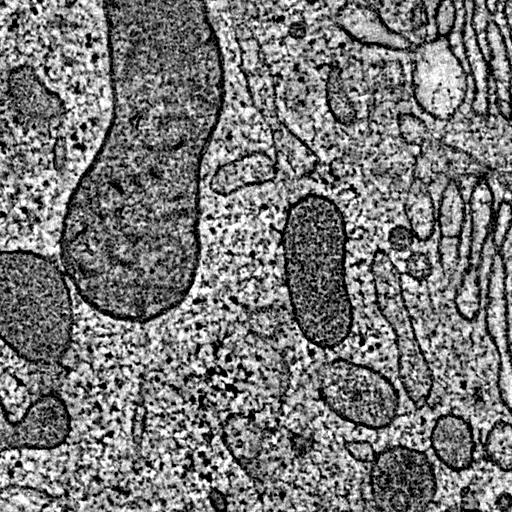
\includegraphics[width=0.49\textwidth]{images/cell}}
  \hfill
  \subfigure[Blurred]{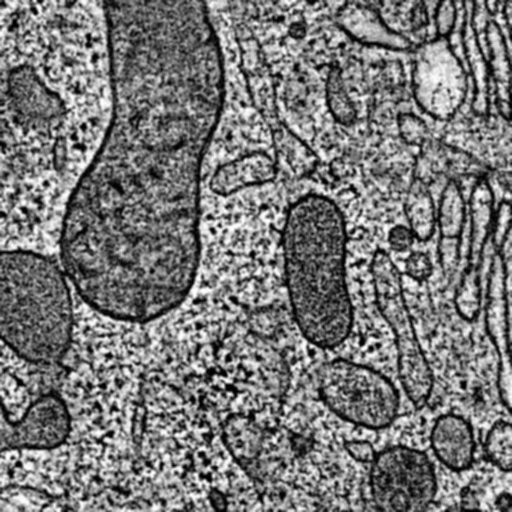
\includegraphics[width=0.49\textwidth]{images/cell_avg}}
  \caption{Example image before and after blurring with average
    filter.\label{fig:eximg}}
\end{figure}

\begin{figure}
  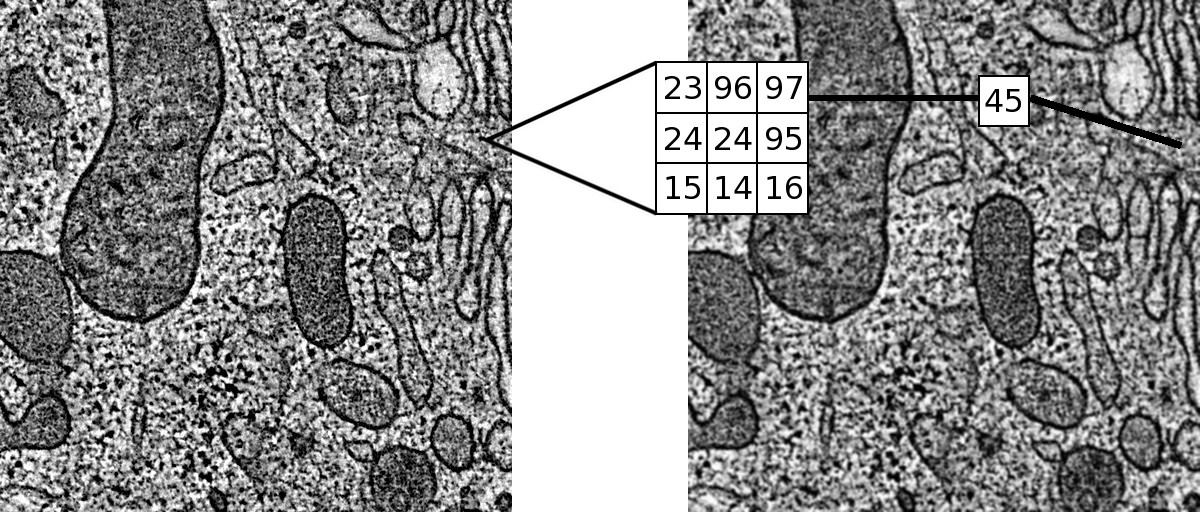
\includegraphics[width=1.0\textwidth]{images/avg_process}
  \caption{Visualising the process of blurring an image using average
    filtering with a 3x3 neighbourhood.\label{fig:exavg}}
\end{figure}

The rest of this section describes how I implemented this, and what
the results where with regards to the performance (how efficient the
implementation is).

\subsubsection{Syntax}

The methods to load and save the image, as well as the \texttt{Square}
definition of structuring element, are all member functions in classes
\texttt{SImageIO} and \texttt{StrElType}. These can be imported with
the \texttt{.\_} notation in Scala, and are then available directly:

\begin{lstlisting}
import io.SImageIO._
import structs.StrElType._

// SImageIO.loadImageCP("/cell.jpg")
val img = loadImageCP("/cell.jpg")
...
saveImage(imgAvg, "/cell_avg.jpg")

// StrElType.Square
val se = StrEl(Square, 3)
\end{lstlisting}

To create the structuring element, the \texttt{StrEl} trait has a
<<companion object>> with an \texttt{apply} method (described in
section \vref{sec:applymethod}. This gives a very compact syntax,
combined with the import of the available structuring element types as
shown above:

\begin{lstlisting}
object StrEl {
  import StrElType._
  def apply(t: StrElType, num: Int) = Array2DStrEl(t, num)
}

val se = StrEl(Square, 3)
\end{lstlisting}

Using traits, we are able to compose image objects with the operations
we want. The operations are implemented in separate traits which are
mixed in with the image on creation. This is using self-type
annotations to specify that the trait can only be mixed in with
classes of type \texttt{GrayScaleImage}:

\begin{lstlisting}
trait Standard { this: GrayScaleImage =>
  def avg(se: StrEl[Int]) = { ... }
}

object Image {
  import operations.{Morphology, Standard}

  def apply(d: Matrix[Int]) = {
    new GrayScaleImage(d) with Standard with Morphology
  }
}

val imgAvg = img.avg(se)

// Equivalent - operator notation
val imgAvg = img avg se
\end{lstlisting}

\subsection{Charting DSL}

TODO: describe DSL utilizing a Java charting library (jfreechart) to
create charting DSL.

A DSL based on the Java library
JFreeChart\footnote{\url{http://www.jfree.org/jfreechart} -- Open
  source (LGPL licensed) charting library written in Java.}.

An example pie chart created with the DSL is shown in figure
\vref{fig:piechartex}.

\begin{figure}
  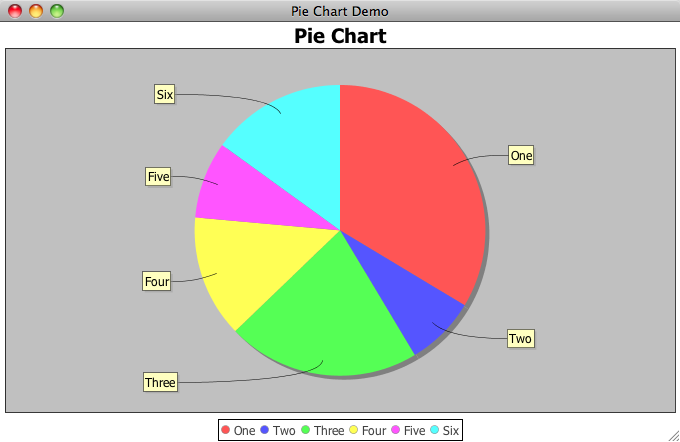
\includegraphics[width=1.0\textwidth]{images/piechart}
  \caption{Example pie chart created with the JFreeChart based
    charting DSL.\label{fig:piechartex}}
\end{figure}

\subsection{Statistics DSL}

TODO: describe simple statistics DSL.

\subsection{Chess DSL}

TODO: describe chess DSL.

\section{Other Examples Used}

This section describes some other DSLs used as examples. They have not
been written as part of the work, but are used as examples as they are
popular DSLs being used.

\subsection{Ruby on Rails}

TODO: describe ruby on rails.

\subsection{Testing Frameworks}

TODO: describe jMock and ScalaTest.

\subsection{Query Languages}

TODO: describe LINQ and related projects on Scala/JVM.

\chapter{Syntax}
\label{sec:syntax}

\textit{The syntax of a language defines its surface
  form.}\cite{fri08} It is the set of rules that define the
combinations of symbols that are considered to be correctly structured
programs in that language. So a DSL is defined in terms of its
syntax. For an embedded DSL its syntax describes special ways to use
the host language. This chapter describes various programming language
concepts that can be useful when designing an embedded DSL. The final
section concludes on some major differences between various classes of
host languages and what these mean to the construction of embedded
DSLs.

\section{Function Chaining/Nesting}
\label{sec:functionchaining}

As mentioned in section \vref{sec:embeddeddsl}, Fowler and Evans have
used the term \texttt{fluent interfaces} to describe libraries that
can be used in a certain way. A key functionality when creating such
fluent interfaces in Java is the ability to chain/nest functions
together.

One of the simplest ways to create a DSL-like syntax is to allow
chaining several function calls together. As an example consider the
following Java-code (from\cite{fow06}), where the construction of a
\texttt{HardDrive} object is shown with and without method chaining:

\begin{lstlisting}[language=java]
// Construct with setter methods
HardDrive hd = new HardDrive();
hd.setCapacity(150);
hd.setExternal(true);
hd.setSpeed(7200);

// Construct with method chaining
HardDrive hd = new HardDrive().capacity(150).external().speed(7200);
\end{lstlisting}

The chaining of methods can also be combined with method nesting,
grouping methods that belong together (also from\cite{fow06}). An
example of this is shown in listing \vref{fig:javachaining}.

\begin{lstlisting}[float,caption=Java method chaining and nesting,label=fig:javachaining,language=java]
computer(
  processor(
    cores(2),
    Processor.Type.i386
  ),
  disk(
    size(150)
  ),
  disk(
    size(75),
    speed(7200),
    Disk.Interface.SATA
  )
);
\end{lstlisting}

In\cite{fre06}, this technique is described in detail. In the testing
framework \texttt{jMock}\footnote{jMock -- A Lightweight Mock Object
  Library for Java: \url{http://www.jmock.org/}} a carefully designed
set of interfaces and factory builder objects allow method chaining
maintaining the wanted order of method calls. The referred paper is a
very good read demonstrating how to design and build a library as an
embedded DSL in Java. The example shown in listing \vref{fig:jmock} is
from this paper, showing the DSL syntax of mock object expectations
used in a mock \texttt{Offer} class.

\begin{lstlisting}[float,caption=Java jMock example,label=fig:jmock,language=java]
void testAcceptsOfferIfLowPrice() {
  offer = mock(Offer.class);
  offer.expects( once() )
       .method( "buy" )
       .with( eq(QUANTITY) )
       .will( returnValue(receipt) );
  ...
}
\end{lstlisting}

Function chaining is available in most programming languages. In
functional programming it is a fundamental concept, while in
object-oriented langauges more a design choice (as in the example
above).

\section{Static Methods/Singleton Objects}

In object-oriented languages functions are nested inside classes. In
order to be able to call functions without instantiating objects we
have static methods, that are associated directly with the class
instance and not with objects created from the class. The following
example shows how to sort a list of strings in Java, using the static
method \texttt{sort} in the \texttt{Collections} class:

\begin{lstlisting}[language=java]
// Create a list of strings
List<String> names = ...

// Sort the list
Collections.sort(names);
\end{lstlisting}

A different approach to static methods is the singleton objects found
in Scala. Instead of having methods defined as static there is a
notion of a singleton object, as in the following example defining
sorting similar to the Java-example above:

\begin{lstlisting}
// Define ListSorter object
object ListSorter {
  def sort(list: List) { ... }
}

// Use object
var names = List("name1", "name2")
ListSorter.sort(names)
\end{lstlisting}

Static methods may play a central role in an embedded DSL, especially
combined with \texttt{Member Imports} (next section). They are
typically used for object creation through patterns like
\texttt{Factory method}\footnote{The factory method is an
  object-oriented pattern that handles the creation of objects without
  specifying the exact class of the object\cite{gam95}.} and
\texttt{Builder}\footnote{The builder pattern is an object-oriented
  pattern that assists the creation of variations of objects through a
  series of abstract method calls\cite{gam95}.}, or other utility operations
like the sorting shown in the examples above. In my image analysis DSL
(described in section \vref{sec:dslimageprocessing}), singleton
objects are used to construct objects:

\begin{lstlisting}
// Using singleton object:
val squareElement = StrEl(Square, 3) // 3x3 square element
val lineElement = StrEl(HLine, 5) // 5x1 line element

// Without singleton object, using new:
val squareElement = new StrEl(Square, 3)
val lineElement = new StrEl(HLine, 5)
\end{lstlisting}

\section{Member Imports}

Member imports is a very useful mechanism in object-oriented languages
for creating concise syntax, and thus in the embedding of DSLs. Using
static member import the Java sorting example from previous section
could have been written like this:

\begin{lstlisting}[language=java]
import static java.util.Collections.*; // Import all static members of the Collections class
...

// Create a list of strings
List<String> names = ...

// Sort the list
sort(names);
\end{lstlisting}

In Scala member imports are less restricted than in Java. They can be
used anywhere in the code (not just at the start of the file), and are
not restricted to static members.

\begin{lstlisting}
class Fruit(val name: String, val color: String) // Define class Fruit with two members

val apple = new Fruit("apple", "red") // Create apple as instance of Fruit

import apple._ // Import all members from object apple

println(name + " is " + color) // Access members 'name' and 'color' directly
\end{lstlisting}

My image processing DSL uses a number of member imports to enable a
concise syntax when working with the DSL, allowing the user of the DSL
to use the method/type names directly (such as the
\texttt{loadImageFile} method and the \texttt{Square} type in the
example below):

\begin{lstlisting}
import simage.io.SImageIO._
import simage.structs._
import simage.structs.StrElType._

val img = loadImageFile("cell.jpg") // Would be SImageIO.loadImageFile without member import
val se = StrEl(Square, 3) // Would be ...StrElType.Square

saveImage(img.avg(se), "cell_avg.jpg") // Would be SImageIO.saveImage without member imports
\end{lstlisting}

\section{Method Names and Operator Notation}
\label{sec:methodnames}

When constructing an embedded DSL we like to make the syntax reflect
the actual domain as much as possible. Having flexible ways to name
and call methods can be a very useful property of a host language.

Scala has two features regarding method names and syntax that are
interesting with regards to DSL development\cite{dub06}:

\begin{itemize}
\item Arbitrary method names - Scala methods can have special
  characters as names. As such Scala has full support for operator
  overloading, as operators are just regular methods with special
  names. For example \texttt{+}, \texttt{!=} and \texttt{<=}.
\item Operator notation - Methods in Scala can be called without the
  dot and parentheses.
\end{itemize}

The following example shows how the operator notation is used together
with the \texttt{+} method name in a simple matrix DSL (being an
important part of the larger image processing DSL shown in section
\vref{sec:dslimageprocessing}):

\begin{lstlisting}
abstract class Matrix {
  // Method names can be operators
  def +(other: Matrix) = add(other)
  // Regular method name
  def add(other: Matrix): Matrix // Abstract method
}

// Usage example - regular notation
val m3 = m1.+(m2)
val m3 = m1.add(m2)
// Operator notation
val m3 = m1 + m2
val m3 = m1 add m2
\end{lstlisting}

Combining the method naming in Scala with method chaining can give
``fluent interfaces'' with even more concise syntax than what was
shown in previous sections. The following example is used from the
website of ScalaTest, as testing framework supporting Behaviour Driven
Development\footnote{BDD is a software development technique first
  introduced in\cite{nor06}. It aims at writing automated tests in a
  natural language, and has been implemented as embedded DSLs in a
  number of different languages.} in a very fluent style:

\begin{lstlisting}
import org.scalatest.FlatSpec
import org.scalatest.matchers.ShouldMatchers

class StackSpec extends FlatSpec with ShouldMatchers {

  "A Stack" should "pop values in last-in-first-out order" in {
    val stack = new Stack[Int]
    stack.push(1)
    stack.push(2)
    stack.pop() should equal (2)
    stack.pop() should equal (1)
  }

  it should "throw NoSuchElementException if an empty stack is popped" in {
    val emptyStack = new Stack[String]
    evaluating { emptyStack.pop() } should produce [NoSuchElementException]
  }
}
\end{lstlisting}

In the dynamic language Ruby they have a similar mechanism as in
Scala. Here you are allowed to leave the parentheses surrounding the
parameter(s) out, but not the dot in front of the method name. In
addition it is a common idiom in Ruby to append method names with a
questionmark if the method returns a boolean value. As shown in the
following example demonstrating how parentheses are optional:

\begin{lstlisting}[language=Ruby]
name = "John"

# Method without parameters
name.empty?()
name.empty?

# Method with one parameter
name.include?("e")
name.include? "e"
\end{lstlisting}

\section{Special Syntax Constructs}

Many programming languages have special constructs that are made
specifically to enable the writing of concise statements. Typically
constructs that only offer a different syntax that will be replaced by
the compiler at early phases of compilation. The next sub-sections
describe some examples of such mechanisms.

\subsection{The ``magic'' \texttt{apply} Method}
\label{sec:applymethod}

Scala uses the \texttt{apply} method to let classes and object define
functionality that appears to be native in the language. You can leave
the method name out and simply write syntax that seems to pass
parameters directly to an object. In the following example the
\texttt{apply} method is used to index the \texttt{Matrix} class as if
it was a native feature:

\begin{lstlisting}
class Matrix[T] {
  def apply(row: Int, col: Int): T = ...
}
val intMatrix = ... // Matrix[Int]
// Get Int at position 2, 4
val intVal = intMatrix(2, 4) // Replaced by compiler: intMatrix.apply(2, 4)
\end{lstlisting}

The \texttt{apply} method can also be used for object construction
without using the \texttt{new} keyword, and without exposing the
actual class being used to create the object. This makes it possible
to create code according to the factory method pattern\cite{gam95}, as
in the following example (simplified version of Matrix structure):

\begin{lstlisting}
abstract class Array2DMatrix[T](elements: Array[T]) extends Matrix[T] {
  ... // Some abstract specialization of the Matrix class
}

class IntArray2DMatrix(elements: Array[Int]) extends Array2DMatrix[Int](elements) {
  ... // Concrete implementation of an int matrix
}

// Singleton object being used to create instances of IntArray2DMatrix
object Matrix {
  def apply(ints: Int*) = new IntArray2DMatrix(Array(elements: _*))
}

// Example use, create matrix from a number of integers - hiding details about the classes shown above
val matrix = Matrix(1, 2, 3, 4, 5, 6, 7, 8)
\end{lstlisting}

As we can see from the above example, combining singleton objects with
the \texttt{apply} method can effectively hide a complex
object-oriented underlying structure. The user of the DSL can focus on
only the details that are relevant (as the list of numbers making up
the matrix in the example above, implementation details being
irrelevant).

\subsection{Query Syntax}
\label{sec:querysyntax}

In C\# 3.0 a DSL called LINQ (Language Integrated Query) was
introduced. It is used to natively query data in the language. The
implementation of the DSL relies on a number of language features
(type inference, anonymous types, object initializer and lambda
expressions -- see sections below) in addition to the query syntax
itself.

\begin{lstlisting}[language={[Sharp]C}]
// Query syntax:
var results = 
  from c in SomeCollection
  let x = someValue * 2
  where c.SomeProperty < x
  select new {c.SomeProperty, c.OtherProperty};

// Resulting rewritten syntax:
var results =
  SomeCollection.Where(
    c => c.SomeProperty < (SomeValue * 2)
  ).Select( c => new {c.SomeProperty, c.OtherProperty} );
\end{lstlisting}

In Scala we have \texttt{for comprehensions} that can be viewed as a
query syntax much like that of LINQ. Complex expressions using the
mechanism will be rewritten to a combination of \texttt{filter},
\texttt{flatMap} and \texttt{map}:

\begin{lstlisting}
// "Query syntax" - for comprehension:
val results = for {
  name <- listOfNames
  if (name startsWith "E")
} yield { name toUpperCase }

// Resulting rewritten syntax:
val results = listOfNames.filter(_ startsWith "E").map(_ toUpperCase)
\end{lstlisting}

Daniel Spiewak has written a paper investigating the possibility to
extend the for comprehensions in Scala to support LINQ-style database
queries\cite{spi09}. Both mechanisms rely on monadic behaviour
(concept from functional programming), where complex statements can be
constructed by combining a set of basic functions (as shown in the
examples above).

\section{Type Inference}

With type inference the compiler will figure out the type of a value
or function, so there is no need to explicitly specify it. This is
useful when writing embedded DSLs, to give a less verbose and more
concise syntax. Some examples were given in the previous section about
query syntax.

The Scala compiler will try to infer the types used. So if the type is
obvious there is no need to specify it:

\begin{lstlisting}
val i = 42 // Type Int is infered
val d = i + 2.1 // Type Double is infered
val iBy2 = (i: Int) => i * 2 // Return value Int is infered from int parameter
val dBy2 = (i: Double) => i * 2 // Return value Double is infered from int parameter
\end{lstlisting}

In the image processing DSL I have made extensive use of the type
inference mechanism. As we can see from the example in listing
\vref{fig:scalatypeinference} there is no explicit naming of the types
involved, as opposed to the bottom part where the same code is given
with the types. As the \texttt{avg} function is specified in the
\texttt{Standard} trait being used with the \texttt{GrayScaleImage}
the full type ``GrayScaleImage with Standard'' must be given, as well
as the \texttt{Int} type parameter to the \texttt{StrEl}. The example
also displays the power in hiding the implementation details from the
user of the DSL.

\begin{lstlisting}[float,caption=Scala type inference example,label=fig:scalatypeinference]
val img = loadImageFile("cell.jpg")
val se = StrEl(Square, 3)
val blurredImg = img.avg(se)

// Without using type inference the code would look like this:
val img: GrayScaleImage with Standard = loadImageFile("cell.jpg")
val se: StrEl[Int] = StrEl(Square, 3)
val blurredImg: Image = img.avg(se)
\end{lstlisting}

\section{Implicit Type Conversion}
\label{sec:implicit_type_conversion}

Implicit type conversions are used to allow the compiler to
automatically convert one type to another where possible. From a DSL
syntax perspective this is used to "add" new methods to existing
types. This can be built-in types or user-defined types. In the
following Scala example an implicit conversion is used to convert from
\texttt{Int} to \texttt{MyInt}, and thus allowing the
\texttt{doubleIt} method to be called directly on the integer value:

\begin{lstlisting}
// Wrapper class for int
class MyInt(val i: Int) {
  def doubleIt = i * 2 // Method
}
// Implicit conversion
implicit def fromInt(i: Int) = new MyInt(i)
// Convert Int to MyInt and call method
val ten = 5.doubleIt
\end{lstlisting}

Implicit conversions are commonly used when creating embedded DSLs in
Scala. A good example if found in the ScalaTest example shown in
section \vref{sec:methodnames}, where the \texttt{String} type is used
as if it had defined the methods \texttt{should} and \texttt{in}. The
value returned from the \texttt{pop} operation on the stack being
tested is treated the same way:

\begin{lstlisting}
...
"A Stack" should "pop values in last-in-first-out order" in {
...
  stack.pop() should equal (2)
  stack.pop() should equal (1)
}

it should "throw NoSuchElementException if an empty stack is popped" in {
...
\end{lstlisting}

What makes this possible is a some implicit conversions. For the
\texttt{String} class the \texttt{should} method is defined in a class
called \texttt{StringShouldWrapper}, which is implicitly available
since there is defined a conversion from \texttt{String}. The value
popped off the stack is converted to a \texttt{AnyShouldMatcher} with
a similar implicit conversion, including a generic type parameter:

\begin{lstlisting}
implicit override def convertToStringShouldWrapper(o: String): StringShouldWrapper

implicit def convertToAnyShouldWrapper[T](o: T): AnyShouldWrapper[T]
\end{lstlisting}

In dynamic languages a mechanism that can give much the same results
is Monkey Patching described in
section \vref{sec:monkey_patching}. Implicit conversions are also very
useful when combining DSLs. This is described in
section \vref{sec:combining_dsls}.

\section{Lambda Expressions/Anonymous Functions}

Anonymous functions, or lambda expressions, can be used as parameters
for higher-order function\footnote{Higher-order functions are
  functions that can take other functions as input parameters or
  return a function as output value.}. They are useful to make concise
code, and avoiding duplication. For example in the Scala for
comprehensions and the LINQ statements shown in section
\vref{sec:querysyntax}, anonymous functions play a role in allowing
filtering (if-statements).

To show how anonymous functions work consider the following
example. The goal is to filter all even numbers from a list, typically
done with the modulo operator (\%). Writing this code in Java, which
does not support anonymous functions, would result in something
similar to this using a \texttt{for-loop} combined with an
\texttt{if-statement}:

\begin{lstlisting}[language=java]
List<Integer> numbers = ... // Make instance of list of integers
List<Integer> evenNumbers = new ArrayList<Integer>();

for(int number : numbers) {
  if(number % 2 == 0) evenNumbers.add(number);
}
\end{lstlisting}

In a language supporting anonymous functions, the \texttt{List} class
could have a \texttt{filter} method taking a function as parameter
which is used to decide what values should be returned in a new
list. In Scala, for example, the above example could be implemented as
follows:

\begin{lstlisting}
val numbers = ... // Make instance of list of integers
val evenNumbers = numbers.filter(_ % 2 == 0)
\end{lstlisting}

It is quite clear that anonymous functions make the code much more
to-the-point and concise. In the Scala example we could leave out both
the loop and the if statement, only focusing on the actual operation
being performed (the modulo 2 equal to 0). If several different
similar operations were to be performed the example would be even
clearer. In Java the loop would have to be repeated several times, or
at least several if-statements would have to be included in the loop,
while in Scala (or other languages supporting anonymous functions) the
operations would occur in an ordered series of filter-statements.

In my Matrix DSL I have used higher-order functions to create
general-purpose functions to perform operations spanning a given
structuring element. The signature looks like this:

\begin{lstlisting}
def seOp(se: StrEl[Int], op: (Seq[T]) => T): Matrix[T]
\end{lstlisting}

It might look cryptical at first, but is really quite simple. The
first parameter is a structuring element (typically spanning a small
3x3 section of the matrix), and the second is a function converting a
sequence of values to one value. The structuring element is passed
over the matrix as a window, and the operation is run for all values
covered by the element. The yielded value is set as a new value in a
new matrix, which is the final return value of the whole function. In
the image processing DSL based on the Matrix DSL this functionality is
used to implement a number of operations, using anonymous
functions. This is shown in listing \vref{fig:scalaanonfunc}.

\begin{lstlisting}[float,caption=Scala anonymous function example,label=fig:scalaanonfunc]
val matrix: Matrix[Int] // Internal image representation as a matrix

// Use average anonymous function to create blur effect
def blur(se: StrEl[Int]) = {
  Image(matrix.seOp(se, (seq) => seq.reduceLeft(_ + _) / seq.size))
}

// Use minimizing anonymous function to create morphological erosion effect
def erode(se: StrEl[Int]) = {
  Image(matrix.seOp(se, (seq) => seq.reduceLeft(_ min _)))
}

// Use maximizing anonymous function to create morphological dilation effect
def dilate(se: StrEl[Int]) = {
  Image(matrix.seOp(se, (seq) => seq.reduceLeft(_ max _)))
}
\end{lstlisting}

These implementations should look familiar to anyone with a knowledge
of image processing, which is the target user domain of the
DSLs. Users of the image processing DSL would never have to see the
anonymous functions, but could use the function \texttt{blur},
\texttt{erode} and \texttt{dilate} directly:

\begin{lstlisting}
val image = ... // Obtain image instance
val se = StrEl(Square, 3) // Create 3x3 structuring element
val blurredImage = image.blur(se)
val erodedImage = image.erode(se)
\end{lstlisting}

Anonymous functions are also available in Ruby, Groovy and
Clojure. They are often referred to/intermixed with
closures\footnote{Closures are actually anonymous functions binding a
  variable defined in a surrounding scope, but the difference is not
  important to the usages described here (or most other places,
  really).} in Ruby and Groovy, and as lambda expressions in
Clojure. Support for anonymous functions has also been discussed for
the next version of Java\footnote{Several different proposals for
  closures/anonymous functions in Java 7 have been discussed. The main
  effort is now lead by Mark Reinhold, as stated on his blog
  (\url{http://cr.openjdk.java.net/~mr/lambda/straw-man/}), and is
  documented as ``Project Lambda'' at the OpenJDK:
  \url{http://openjdk.java.net/projects/lambda/}.}.

\section{Anonymous Types}

Anonymous types allow the construction of types without a name, based
on fields. Combined with type inference this is a central feature in
the implementation of LINQ (as described in an earlier section).

Scala also supports anonymous types. An example of using anonymous
types together with type inference:

\begin{lstlisting}
val person = new { val name = "John"; val age = 26 }

println(person.name + " is " + person.age + " years old..")
\end{lstlisting}

In LINQ this is used to allow selection of fields from a database or
other data structure:

\begin{lstlisting}[language={[Sharp]C}]
var results = 
  ... // Some query
  select new {c.SomeProperty, c.OtherProperty};
\end{lstlisting}

\section{Object Initializer}

Object initializers provide the ability to give values to an object
while instantiating it. In C\# this can look like the following, and
is also used to select objects of given class instead of anonymous
types from LINQ:

\begin{lstlisting}[language={[Sharp]C}]
val results =
  ... // Some query
  select new Person { Name = c.SomeProperty, Age = c.OtherProperty }
\end{lstlisting}

Scala also supports a form for object initializers, as in the
following example:

\begin{lstlisting}
class Person {
  var name = ""
  var age = 0
}

val person = new Person { name = "John"; age = 26 }
\end{lstlisting}

\section{Metaprogramming}

Metaprogramming is the writing of computer programs that write or
manipulate other programs (or themselves) as their data, or that do
part of the work at compile time that would otherwise be done at
runtime. In terms of embedded DSL creation, metaprogramming can be an
extremely useful mechanism. There are quite drastic differences
between the different programming paradigms how they solve
metaprogramming, how it is used and what you can do with it. The next
sub-sections describe some of these differences with examples.

\subsection{Metaprogramming in Static Languages}

Java has a wide range of mechanisms associated with metaprogramming:

\begin{itemize}
\item Annotations -- Annotations were introduced to Java with version
  5 (JDK 1.5). They are used to add metadata about a program. These
  data are not part of the program itself, and can be used both at
  compile-time/deployment-time and at runtime. Deployment-time
  annotations can be used for code generation, and can be used when
  embedding DSLs.
\item Reflection -- Reflection is a way to program with concepts such
  as \texttt{class} and \texttt{method} in Java, and as such is
  considered a form of metaprogramming. Extensive use of reflection
  can have a negative effect on the performance of a Java application.
\item Aspect Oriented Programming (AOP) -- AOP has become a popular
  mechanism in many Java frameworks the last years. It is too big of a
  concept to describe in detail here, but is worth mentioning in the
  light of metaprogramming. With AOP it is possible to alter the
  behaviour of Java-code dramatically. I have, however, not looked
  detailed at AOP here as it is not really part of the Java
  language\footnote{Aspect Oriented Programming is usually implemented
    by pre-compilation, or extensive use of dynamic proxies in
    Java. Some of the most popular AOP frameworks in Java are AspectJ
    (\url{http://www.eclipse.org/aspectj/}), JBossAOP
    (\url{http://www.jboss.org/jbossaop}) and Qi4j
    (\url{http://www.qi4j.org/}).}.
\end{itemize}

As an example of an embedded DSL in Java relying heavily on
annotations is the Hibernate framework, providing an object-relational
mapping between Java domain objects and database tables. The example
in listing \vref{fig:javameta} shows Hibernate in work mapping the
classes \texttt{Person} and \texttt{Address} to database tables. A
person has one address, but many persons can live on the same
address. This relationship is mapped using annotations. With these
annotations in place, Hibernate will generate the mapping (SQL-code)
needed to extract correct data from the database.

\begin{lstlisting}[float,caption=Java metaprogramming with annotations,label=fig:javameta,language=java]
@Entity
public class Person {
  @Column(name="person_name", length=100)
  public String getName() { ... }

  @ManyToOne
  public Address getAddress() { ... }
}

@Entity
public class Address {
  ...
  @OneToMany
  public List<Person> getPersons() { ... }
}

// Example of use
Address adr = ... // obtain some address object
// The getPersons() method will actually run some SQL in the background fetching correct persons
for(Person person : adr.getPersons()) { ... }
\end{lstlisting}

Scala has no special mechanism for metaprogramming yet, and has not
been considered in this section.

\subsection{Dynamic Metaprogramming}

Dynamically typed languages are able to use metaprogramming in a more
dynamic way, to add or alter method definitions at runtime. Both
Groovy and Ruby have powerful support for this kind of dynamic
metaprogramming.

The example in listing \vref{fig:groovymeta} shows how the mechanism
can be used. In this case a new method is added to the Java
\texttt{String} class\footnote{Note that the \texttt{String} class is
  final in Java, but still modifiable with dynamic metaprogramming in
  Groovy.}, and the static \texttt{random} method of the \texttt{Math}
class is changed to a not-so-random implementation useful for unit
testing or other environments where you want to have full control of
returned values:

\begin{lstlisting}[float,caption=Groovy metaprogramming example,label=fig:groovymeta,language=java]
// Add a "shout" method to the Java String class
String.metaClass.shout = {
  println delegate.toUpperCase()
}
"hello".shout() // prints "HELLO"

// Handy when you want to do controlled unit testing?
Math.metaClass.static.random = {
  return 42
}
\end{lstlisting}

The implementation is roughly the same in Ruby. A typical example of a
DSL utilizing metaprogramming is the Rails framework and the
\texttt{ActiveRecord} class. Here metaprogramming is used to specify
relationships between the classes, with respect to database
relationships. The SQL code needed to fetch related objects will be
generated as new methods. In the example in listing
\vref{fig:railsmeta} this technique is shown for the classes
\texttt{Team} and \texttt{Player}. The methods \texttt{has\_many} and
\texttt{belongs\_to} are implemented in a manner similar to the Groovy
examples above, adding methods \texttt{team} and \texttt{players} with
database extraction logic to the classes in use.

\begin{lstlisting}[float,caption=Ruby on Rails example showing dynamic metaprogramming,label=fig:railsmeta,language=Ruby]
class Team < ActiveRecord::Base
  has_many :players
end

class Player < ActiveRecord::Base
  belongs_to :team
end

# Now a player will have a 'team' method returning the team
player.team

# And a team will have a 'players' method returning a collection of players
team.players.each { |team| ... }
\end{lstlisting}

A simplified example of how the \texttt{belongs\_to} method is
implemented using dynamic metaprogramming is shown in listing
\vref{fig:rubydynmeta}, running some SQL and creating a collection of
associated object dynamically.

\begin{lstlisting}[float,caption=Ruby dynamic metaprogramming example,label=fig:rubydynmeta,language=Ruby]
class ActiveRecord
  ...
  def self.has_many(arg)
    name = arg.to_s
    send :define_method, name do
      sql = "select * from #{name} where #{self.class.name.downcase!}_id = #{self.object_id}"
      # Run sql, and return new objects based on sql result
      ...
    end
  end
  ...
end
\end{lstlisting}

This dynamic style metaprogramming is one of the biggest advantages
dynamic languages have when it comes to designing embedded DSLs. Using
annotations or other metaprogramming techniques could be used in Java
or other static languages to generate code similar to the one
generated by the rails framework. However, the client would not know
about the methods until after compiling. So programming in this
fashion in a static language would require some intermediate step of
explicit code-generation or compiling before calling the generated
methods. I think this is an extremely big differenciator when it comes
to certain kind of DSLs and programming language paradigms. A DSL like
Rails could never have been written in a static language.

\subsection{Functional Metaprogramming}

In Clojure, the only ``pure'' functional language used in this thesis,
there is no big separation between code and data. As such the whole
concept of metaprogramming is really just an integrated part of the
language, and not necessarily seen as a ``different'' concept (as in
the other languages). The macro mechanism in Clojure is the key to this.

TODO: describe Clojure macros. Syntax quote, unquote and splicing
unquote.

Clojure also has some explicit functions to work with metadata --
\texttt{meta} and \texttt{with-meta}. Some examples of use are shown
in code listing \vref{fig:clojuremeta}.

\begin{lstlisting}[float,caption=Clojure metaprogramming example,label=fig:clojuremeta,language=lisp]
(def my-user {:login "test" :password "secret"})      
; #'user/my-user
my-user
; {:login "test", :password "secret"}
(meta my-user)
; nil
(def my-cached-user (with-meta my-user {:cached-at (java.util.Date. )}))
; #'user/my-cached-user
my-cached-user
; {:login "test", :password "secret"}
(meta my-cached-user)
; {:cached-at #<Date Sat Feb 06 20:38:28 CET 2010>}
\end{lstlisting}

\section{Open Classes/Monkey Patching}
\label{sec:monkey_patching}

A monkey patch is a way to extend or modify the runtime code of
dynamic languages without altering the original source code. In DSL
creation this can be used in much the same way as implicit
conversions, by adding new functionality to built-in or other
types. In the following code we re-implement with open classes/monkey
patching the same example shown earlier with implicit type
conversions:

\begin{lstlisting}[language=Ruby]
class Integer
  def doubleIt
    self * 2
  end
end

ten = 5.doubleIt
\end{lstlisting}

\section{Dynamic Dispatch -- Method Missing}

Dynamic programming languages use dynamic dispatch to determine what
code to run when a message is received. This means that errors related
to missing methods are postponed until runtime. Some languages provide
interesting ways to handle these errors, that can be utilized in DSL
creation.

In Ruby there is a notion of custom dispatch behaviour that can be
controlled by the programmer. The base class, that all other classes
extend from, has a \texttt{method\_missing} method that is called by
the dispatcher as a last resort when no other method is found to
respond to a message. The default behaviour is to throw a
\texttt{NoMethodError}, but this can be overridden by extending
classes.

To see how this can be used in a DSL we can look at a simplified
version of the \texttt{ActiveRecord} class from the \texttt{Rails}
framework. It maps objects to database tables and allows dynamic
querying through the DSL syntax:

\begin{lstlisting}[language=Ruby]
class ActiveRecord
  # ...
  def self.method_missing(method_id, *arguments)
    if match = /find_(all_by|by)_([_a-zA-Z]\w*)/.match(method_id.to_s)
      # ... extract column names from match, generate and run SQL expression + map and return results
    end
  end
end

# Define class 'Person' as extension of 'ActiveRecord'
class Person < ActiveRecord::Base
end

# Query the database for person with given username
person = Person.find_by_username "eivindw"
\end{lstlisting}

\section{Summary}

Modern statically typed languages like Scala offer some very powerful
features for building embedded DSLs, combining concepts from
object-oriented and functional programming languages. Advanced type
systems offering type interference, implicit conversions and anonymous
types provide powerful mechanisms when constructing DSLs, removing
much of the verbosity often associated with statically typed
languages.

When comparing various classes of programming languages the biggest
difference with regards to DSL syntax seems to be that between static
and dynamic languages. Even with feature rich static programming
languages like Scala there are a series of concepts from dynamic
languages which does not have a natural counterpart in the statically
typed domain. Most notebly are the powerful metaprogramming features
found in many dynamic languages and the dynamic dispatch mechanism
allowing custom handling of missing methods.

\chapter{Composition}
\label{sec:composition}

This chapter looks at various composition techniques used when working
with DSLs. It is divided into two main sections; the first one
describing how modular composition can be useful when constructing a
single DSL, and the second showing how to combine multiple DSLs to
create new ones.

\section{Modular DSL Composition}

With modular composition I mean structuring a program such that the
implementation is spread over several separate modules. A modular
design can be useful when creating a DSL. With a loosely coupled
modular implementation the DSL can easily be extended by implementing
new modules, or customized by specifying a subset of modules to be
included. In the following subsections two different ways to create a
modular composition is shown and discussed. First an object-oriented
technique involving mixin-composition using traits is shown, and
secondly functional composition using decorators is shown.

\subsection{Traits - Polymorphic Abilities}

Scala has support for virtual types (abstract type members) and
familiy polymorphism\cite{ode03}, mixin composition\cite{ode05} and
higher-order genericity\cite{moo08}. These are all powerful features
that support polymorphic embedding of DSLs\cite{hof08}.

This allows building DSLs that can have several different
interpretations as reusable components. It can also be used to
effectively combine different DSLs into new ones. The paper
``Polymorphic Embedding of DSLs''\cite{hof08} describes this in detail
with examples.

A use of traits can be to split functionality in several traits and
create classes/objects with only the methods that we need. In the
example given in listing \vref{fig:scalatraits} the \texttt{Matrix}
class does not have any methods, but instances of the class can be
mixed in with traits containing various methods.

\begin{lstlisting}[float,caption=Scala traits example,label=fig:scalatraits]
class Matrix {} // No methods

trait AvgMtx { this: Matrix =>
  def avg(): Matrix = { ... }
}

trait MorphMtx { this: Matrix =>
  def erode(): Matrix = { ... }
  def dilate(): Matrix = { ... }
}

// Matrix with only avg() method
val m1 = new Matrix with AvgMtx
// Matrix with erode() and dilate() methods
val m2 = new Matrix with MorphMtx
// Matrix with "all" methods
val m3 = new Matrix with AvgMtx with MorphMtx
\end{lstlisting}

Mixin composition is also available in Groovy and Ruby. In Groovy
there is a general mixin meta-class function available, making it
possible to combine several classes into one. Because of the dynamic
typing the \texttt{name} variable of the \texttt{Base} class is
available in the mixin-classes, as if they were subclassing the base
class. This is shown in listing \vref{fig:groovymixins}.

\begin{lstlisting}[float,caption=Groovy mixing composition example,label=fig:groovymixins,language=java]
class Base {
  String name;
}

class StdOp {
  def std() {
    println("std() running.." + name);
  }
}

class ExtraOp {
  def extra() {
    println("extra() running.." + name);
  }
}

Base.class.mixin(StdOp, ExtraOp);

base = new Base(name: 'Test!');
base.std(); // Base has a std() function
base.extra(); // ..and an extra() function
\end{lstlisting}

In Ruby there is a \texttt{module} concept that provides dynamic mixin
composition functionality similar to that shown above in
Groovy. Modules are a way to logically group classes, functions or
other definitions belonging together, as an advanced form of the
packages found in Java and Scala. Modules cannot be instantiated like
classes, but can be mixed in with a new or existing class to add
functionality. Given in listing \vref{fig:rubymodules} is the same
example as was shown for Groovy above, implemented using modules in
Ruby.

\begin{lstlisting}[float,caption=Ruby mixin composition using modules,label=fig:rubymodules,language=ruby]
class Base
  @name
  
  def initialize(name)
    @name = name
  end
end

module StdOp
  def std
    puts "std() running.." + @name
  end
end

module ExtraOp
  def extra
    puts "extra() running.." + @name
  end
end

class MyBase < Base
  include StdOp, ExtraOp
end

base = MyBase.new("Test!")
base.std() # MyBase has a std() function
base.extra() # ..and an extra() function
\end{lstlisting}

Using the modular composition techniques it is possible to extract
parts of a DSL as a new one, by only including the traits (or modules)
wanted. An optimizing compiler could also utilize this composition to
only include the parts of a DSL that are actually used, thus
optimizing the size of the bytecode produced.

\subsection{Functional Composition}

TODO: write with clojure examples

\begin{itemize}
\item Multimethods with \texttt{defmulti} and \texttt{defmethod}.
\item Metaprogramming
\item Macro decorators
\end{itemize}

\section{Combining DSLs}
\label{sec:combining_dsls}

This section describes how to combine two DSLs into a new one, mixing
the functionality of the two original DSLs.

\subsection{Implicit Conversion}

Implicit type conversions were described in section
\vref{sec:implicit_type_conversion}, in terms of DSL syntax. In this
section we will look at how implicits can be used to combine
functionality from two different DSLs. The concept is demonstrated
with an example.

The following code shows a simple DSL for statistics in use. Typically
some kind of dataset is created with numeric values (in this example
only integer values for simplicity). The dataset implements the
methods \texttt{average}, \texttt{minValue} and \texttt{maxValue}. In
the most basic form it can be used directly to compute the average,
minimum and maximum values of a series of integers:

\begin{lstlisting}
val ds = DataSet(1, 2, 3, 4, 5, 6, 7, 8, 9)

println("Average: " + ds.average) // 5.0 (double value)
println("Minimum value: " + ds.minValue) // 1 (int value)
println("Maximum value: " + ds.maxValue) // 9 (int value)
\end{lstlisting}

As a first example of using implicit conversion to apply a DSL to new
values, we want to compute statistic values for an array of words
(strings) using the dataset DSL. In the following example an implicit
conversion from string-array to dataset is utilized to find the
average, minimum and maximum word lengths. The dataset is created
using the length of the strings as input, in the implicit function
\texttt{str2DS}. It is then possible to call dataset methods on the
string-array as if it was an instance of a dataset (which in fact it
is as the compiler implicitly converts it to one on demand):

\begin{lstlisting}
val words = Array("eivind", "test", "oslo", "bekk", "scala", "elephant", "cat")

implicit def str2DS(str: Array[String]) = {
  DataSet(str.map(_.length): _*)
}

println("Average: " + words.average) // 4.86 is the average word length
println("Minimum value: " + words.minValue) // 3 is the length of the shortest word
println("Maximum value: " + words.maxValue) // 8 is the length of the longest word
\end{lstlisting}

Finally we combine the image processing DSL with the statistics DSL
using the same technique that was shown for the string-array above. An
implicit conversion is defined converting instances of
\texttt{GrayScaleImage} (image storing only one integer value per
pixel) to a dataset, making it possible to call the statistics method
to compute the average, minimum and maximum pixel values. In a way one
could say that we have defined a new ``statistical image processing
DSL'' combining the two existing DSL, all without writing any other
code than the actual conversion. A simple example is shown below:

\begin{lstlisting}
val img = Image(Matrix(3, List(
  9, 8, 7,
  6, 5, 6,
  7, 8, 9)))

implicit def img2DS(img: GrayScaleImage) = {
  DataSet(img.data.toArray: _*)
}

println("Average: " + img.average) // 7.22 is the average pixel value
println("Minimum value: " + img.minValue) // 5 is the smallest pixel value
println("Maximum value: " + img.maxValue) // 9 is the biggest pixel value
\end{lstlisting}

As with the string-array example shown previously we see how easy it
is to mix in the functionality of one DSL with another. One could
imagine a whole environment built from small DSLs, each describing a
specialized part of the domain. For example an environment for various
numeric analysis could be built combining DSLs for image processing,
statistics, charting etc.

\section{Summary}

TODO: Write conclusion.

\chapter{Advanced Techniques}
\label{sec:advancedtechniques}

This chapter describes some advanced techniques that can be used in
DSL construction. More specifically it deals with operations that
remove functionality from the host language (pruning), and various
ways to extends the host language. One could discuss how relevant this
is when talking about embedding DSLs, as using these techniques widely
can alter the host languages radically. As such an embedded DSL in a
host language can be rendered to act as an external DSL, tweaking the
programming language to suit our needs.

\section{Removing from Host Language -- Pruning}

\subsection{Compiler Plugins}

TODO: example Scala compiler plugin, removing for comprehension
support or similar from the language.

\subsection{Pruning in Dynamic Languages}

TODO: describe how open classes in Ruby can be used
(remove\_method/undef\_method). Groovy possibilities?

\subsection{Pruning in Functional LISP}

TODO: describe possibilities in Clojure.

\section{Extending Host Language}

\subsection{Compiler Plugins}

TODO: Scala compiler plugin example, again?

\subsection{Dynamic Languages}

TODO: Ruby open classes again.

\subsection{Functional Languages}

With functional languages it is possible to create control structures
that look like built-in keywords, but are simply first-class
functions. In Scala functions can be defined with ``pass by name''
parameter passing, and single parameter functions can be called using
curly braces instead of parenthesis to specify the parameter. As an
example consider the following definition of a new while construct:

\begin{lstlisting}
def mywhile(cond: => Boolean)(body: => Unit) {
  if(cond) {
    body
    mywhile(cond)(body)
  }
}

// Example use:
var i = 0
mywhile(i < 3) {
  println("Num: " + i)
  i = i + 1
}
\end{lstlisting}

As we can see it is simple to define functions that act and look like
built-in control structures. This is very useful designing DSLs where
we want it to seem like the host language has been extended with new
features supporting the DSL.

TODO: DSL example using the technique shown above.

TODO: Clojure macro examples.

\section{Summary}

TODO: Write conclusion.

\chapter{Using the DSL}
\label{sec:dsluse}

So far the focus has been on the creation of embedded DSLs. This
chapter discusses various ways to use the DSLs created. There are
quite many ways to take advantage of the DSLs, depending on what kind
of language it has been written in. The next sections describe some of
the usages I have found, and how they are supported by the different
languages.

\section{API/Library}

The most common way to use an embedded DSL seems to be as a library
integrated in other application code. On the JVM this will typically
involve archiving compiled class files, or script + interpreter, in
one or more jar (Java Archive) files. These files will be included in
the classpath of the application that needs access to the library
API. The application programmer will then be able to import the
classes and use in the program code. An example is the JMock framework
in Java (also mentioned in section \vref{sec:functionchaining}). It
allows programmers writing unit tests to specify with an internal DSL
syntax how they want to mock dependencies to the code they are
testing. An example written in Java (DSL syntax mostly found in the
expectations declarations) is shown in listing \vref{fig:javaapi}.

\begin{lstlisting}[float,caption=Java example using jMock as an API,label=fig:javaapi,language=java]
import junit.framework.TestCase;

import org.jmock.Mockery;
import org.jmock.Expectations;

public class PublisherTest extends TestCase {

  public void testSimplePublish() {
    Mockery context = new Mockery();
    Subscriber subscriber = context.mock(Subscriber.class);
    Publisher publisher = new Publisher();
    publisher.add(subscriber)
    String message = "message";
    context.checking(new Expectations() {{
      oneOf(subscriber).receive(message);
      allowing(subscriber).isAlive(); will(returnValue(true);
    }});
    publisher.publish(message);
    context.assertIsSatisfied();
  }
}
\end{lstlisting}

Another interesting thing when using the DSL as a library, is that the
language using the DSL not necessarily needs to be the same as the
host language the DSL was written in. If the DSL is compiled to
bytecode (\texttt{.class} files), it can be used from most of the
other languages running on the JVM. The example above could just as
well have been written in any of the languages used in this thesis,
for example in Scala as shown in listing \vref{fig:scalaapi} (looking
quite similar to the original Java example above).

\begin{lstlisting}[float,caption=Scala example using jMock as an API,label=fig:scalaapi]
import junit.framework.TestCase

import org.jmock.{Mockery, Expectations}

class PublisherTest extends TestCase {

  def testSimplePublish {
    val context = new Mockery
    val subscriber = (context.mock(classOf[Subscriber])).asInstanceOf[Subscriber]
    val publisher = new Publisher
    publisher.add(subscriber)
    val message = "message"
    context.checking(new Expectations {
      oneOf(subscriber).receive(message)
      allowing(subscriber).isAlive; will(returnValue(true)
    })
    publisher.publish(message)
    context.assertIsSatisfied
  }
}
\end{lstlisting}

\section{Scripting}

A different approach to the use-as-a-library approach shown above is
to allow code written in the DSL to be run as a standalone
script. That is without the need to wrap it in some class or module
written in the host language. All the dynamic and interpreted
languages support this kind of usage. Scala, although it is a static
and compiled language, has a kind of interactive interpreter called
REPL (Read-Evaluate-Print Loop) that typically can be used to test
code on the fly. It can also be used to run Scala-code in a more
script-like way. The following script can be run demonstrating this
functionality, using the image analysis DSL from
chapter \vref{sec:examples} as example (loading an image and saving a
blurred copy to a new file):

\begin{lstlisting}
import simage.io.SImageIO._
import simage.structs._
import simage.structs.StrElType._

val img = loadImageFile("cell.jpg")
val se = StrEl(Square, 3)

val blurredImg = img.avg(se)
saveImage(blurredImg, "cell_blurred.jpg")
\end{lstlisting}

The script can then be run from the commandline using the scala
interpreter (called with the \texttt{scala} command), assuming the
script is in a file named \texttt{ImageScript.scala} and that the
image analysis DSL has it's classes packed in the jar
\texttt{simage.jar}:

\begin{lstlisting}[language=]
scala -classpath simage.jar ImageScript.scala
\end{lstlisting}

For users of the image analysis DSL this means a great simplification
in the way it is run. They do not have to learn how to make classes,
objects and methods in Scala, as they would if they wanted to run the
DSL as a regular library in a Scala file (requiring at a minimum
creating an application object with a main method). As image analysis
experts are not necessarily computer programmers this might be a good
idea.

Similar examples can be given for other DSLs and using other host
languages supporting running code as a script.

\section{Interactive Console -- Interpreter}

Many of the programming languages studied have some sort of
interactive interpreter (like the Scala REPL mentioned in the previous
section). This can in many cases be configured to be used with a
specific library pre-loaded, which means it is possible to create a
custom version for working interactively with a DSL. Similar to the
scripting example shown above this opens possibilities to work with
the DSL without wrapping it in any host language code. But the main
advantage of using the DSL in an interactive console is the unique
ability it offers in issuing commands that are run directly.

The Scala REPL has an option to pre-load a file with commands on
startup. Typically this can be used to include imports, implicit
definitions, type aliases or function definitions. Taking the example
from the previous section on scripting we can put all the import
statements into a file called PreDef.scala:

\begin{lstlisting}
import simage.io.SImageIO._
import simage.structs._
import simage.structs.StrElType._
\end{lstlisting}

The interactive interpreter can then be started using the option
\texttt{-i PreDef.scala} as in the following example:

\begin{lstlisting}[language=]
scala -classpath simage.jar -i PreDef.scala

Loading Predef.scala...
import simage.io.SImageIO._
import simage.structs._
import simage.structs.StrElType._

Welcome to Scala version 2.7.7.final (Java HotSpot(TM) 64-Bit Server VM, Java 1.6.0_17).
Type in expressions to have them evaluated.
Type :help for more information.

scala> 
\end{lstlisting}

We can the issue the same commands used in the script example one by
one (notice the output for every line wich is simply the interpreter
calling the \texttt{toString} method after printing the type on the
newly created object -- very useful for debugging purposes):

\begin{lstlisting}[language=bash]
scala> val img = loadImageFile("cell.jpg")
img: simage.structs.GrayScaleImage with simage.operations.Standard with simage.operations.Morphology =
Image 512x512

scala> val se = StrEl(Square, 3)
se: simage.structs.StrEl[Int] = 
Array2D rows:3 cols:3
Array(1, 1, 1, 1, 1, 1, 1, 1, 1)

scala> val blurredImg = img.avg(se)
blurredImg: simage.structs.GrayScaleImage with simage.operations.Standard with simage.operations.Morphology =
Image 512x512

scala> saveImage(blurredImg, "cell_blurred.jpg")

scala>
\end{lstlisting}

From Scala version 2.8\footnote{To be released in the first part of
  2010, available as a first Beta version as of this writing.} the
REPL will have many improvements such as code completion (of
package/class/member names) and interactive debugging.

TODO: Clojure REPL (with user.clj example). Ruby irb. Groovy groovysh
(Groovy Shell).

TODO: check JLine with interpreter (specially Clojure).

\section{Embedded Interpreter}

If we want to take the interactive interpreter in Scala a step further
it is actually possible to embed it in your own
application\footnote{See\cite{sur09} and\cite{dic09} (internet blog
  posts) for examples of how to embed the Scala REPL.}. This could be
a very powerful way to create a standalone application having a
console or similar being able to run DSL commands directly. For the
image analysis example shown in chapter \vref{sec:examples} it would
be possible to create some kind of application combining such a
console with an image viewer window showing the results of the
operations directly on an image. This is similar to how \matlab{}
works, a proven environment for image analysis and other mathematical
calculations.

I think this technique could be very useful for a number of cases. All
kinds of DSLs where you might want to see some immediate results of
your commands could be candidates. Examples could typically be
statistical, financial or graphical DSLs. A generic application might
even be reused for several different DSLs, thus being a powerful base
for building custom running environments for any embedded DSL written
in Scala (or any other language that compiles to regular Java
bytecode).

TODO: example embedding interpreter, with simple Swing gui or similar?

\section{Tool Support}

Since working with an embedded DSL to a large extent means dealing
with a host language, I think it is interesting to provide a brief
overview and comparison over the development tool support the various
languages offer.

\begin{itemize}
\item Java -- IntelliJ, Eclipse, NetBeans++ Refactoring. Code
  completion. Error highlighting. Integration with frameworks.
\item Scala
\item Clojure
\item Ruby -- dynamic language different than static?
\item Groovy
\end{itemize}

\section{Error Handling}

How well does the different host languages support custom error
handling on the DSL level? Separate/different chapter? Compile-time
error handling. Dynamic versus static typing (type-safety).

\section{Summary}

TODO: Write conclusion.

\chapter{Performance}
\label{sec:performance}

This chapter looks at the performance aspects of the various DSLs and
host languages. The categories of languages are compared with regards
to performance, and some example DSLs that depend on high throughput
are implemented and analyzed. The chapter concludes with some key
points to consider when dealing with DSLs that need to run as fast as
possible on the JVM.

\section{Host Language -- Dynamic vs. Static Typing}

TODO: finish section

Performance benchmarks dynamic vs static, interpreted vs compiled,
functional vs object-oriented/imperative.

\section{Code Efficiency}

\begin{itemize}
\item Scala for comprehensions --> while loops - functional
  programming problem on the JVM?
\item Primitives - byte, int and double support - contrast to objects
  on everything (autoboxing)
\item Data structures - Scala list of lists vs 2D-array
\end{itemize}

\subsection{Efficient Implementation Tips}
\label{sec:effimpl}

When performing the same operation a large number of times, as is the
case with many algorithms for Image Processing, there are various
implementation related things that need to be considered. In this
section I summarize the lessons learned with regards to tuning the
code for maximum performance.

\subsubsection{Choice of data structures}
\label{sec:datastructures}

The underlying data structure for images and Image Processing is the
matrix. Since Scala does not include an efficient implementation of
matrix I ended up testing a few different variants:

\begin{itemize}
\item \textbf{List of Lists} -- A very logical implementation of
  matrix is by using Scala \texttt{Lists}. The idea for this
  implementation was inspired by a blog post by Jonathan
  Merritt\cite{mer08}. A simple example of using a list of lists is
  shown in figure \vref{fig:listoflist}. However, this implementation
  proves to be very slow in specific element access and iteration.
\item \textbf{2D Array} -- In Scala an \texttt{Array} will usually be
  faster than \texttt{List} because it is compiled to a native array
  in bytecode. It is also faster to implement as one flat array,
  rather than an array of arrays. This gives a much more efficient
  implementation with regards to element access and iteration. The
  implementation becomes slightly less straight-forward as we need to
  calculate the element positions in the array, as shown in figure
  \vref{fig:2darray}.
\end{itemize}

\begin{lstlisting}[float,caption=Matrix implementation based on List of Lists.,label=fig:listoflist]
class Matrix[T](val elements: List[List[T]]) {
  val nRows = elements.size
  val nCols = if(elements.isEmpty) 0
              else elements.head.size

  require(elements.forall(_.length == nCols))

  def apply(row: Int, col: Int): T = elements(row)(col)
}

val m = new Matrix(List(List(1, 2), List(3, 4)))
\end{lstlisting}

\begin{lstlisting}[float,caption=Matrix implementation based on 2D Array.,label=fig:2darray]
class Matrix[T](cols: Int, val elements: Array[T]) {
  require(elements.size % cols == 0)

  val nRows = elements.size / cols
  val nCols = cols

  def apply(row: Int, col: Int): T = elements(col + row * nCols)
}

val m = new Matrix(2, Array(1, 2, 3, 4))
\end{lstlisting}

\subsubsection{Iterations -- \texttt{for} comprehensions vs \texttt{while} loops}

Many Image Processing operations require some kind of calculation
performed for every element in the underlying matrix. As an example,
consider the neighbour average operation implemented using a general
structuring-element operation show in figure
\vref{fig:strelavg}. Having as efficient implementation of the
\texttt{seOp} method as possible is critical for large matrices. So
having some way of efficiently iterating over all elements of the
matrix is essential. Scala provides two basic forms of iterating;
\texttt{for comprehensions} and \texttt{while loops}:

\begin{itemize}
\item \textbf{for comprehensions} -- In Scala, for comprehensions are
  implemented as a monadic combination of the methods \texttt{filter},
  \texttt{map} and \texttt{flatMap}. This is a very powerful structure
  allowing compact and readable code. An example of implementing a
  general structuring-element operation based on for comprehensions is
  show in figure \vref{fig:forcomp}.
\item \textbf{while loops} -- For regular loops Scala provides the
  \texttt{while} keyword. Using this instead of the for comprehensions
  gives a much more iterative implementation, as shown in figure
  \vref{fig:whileloop}.
\end{itemize}

\begin{lstlisting}[float,caption=Implementing matrix neighbour average using a general structuring-element operation.,label=fig:strelavg]
class Matrix ... {
  def seOp(se: Matrix, op: (Seq[Int]) => Int) = { ... }
}

val matrix = ... // Create matrix - load image or similar
val se = new Matrix(3, Array.make(9, 1))
val avgMatrix = matrix.seOp(se, (seq) => seq.reduceLeft(_ + _) / seq.size)
\end{lstlisting}

\begin{lstlisting}[float,caption=Implementation of a structuring element operation on a matrix using \texttt{for comprehensions}.,label=fig:forcomp]
def seOp(se: Matrix, op: (Seq[Int]) => Int) = {
  val w = se.nCols / 2
  val h = se.nRows / 2

  def seValues(row: Int, col: Int) = {
    for {
      x <- -w to w
      cx = col + x
      y <- -h to h
      ry = row + y
      if(cx >= 0 && cx < nCols && ry >= 0 && ry < nRows)
    } yield {
      elements(cx + ry * nCols)
    }
  }
  val range = for(i <- 0 until nRows; j <- 0 until nCols) yield {
    op(seValues(i, j))
  }
  new Matrix(nCols, range.toArray)
}
\end{lstlisting}

\begin{lstlisting}[float,caption=Implementation of a structuring element operation on a matrix using \texttt{while loops}.,label=fig:whileloop]
def seOp(se: Matrix, op: (Seq[Int]) => Int) = {
  val w = se.nCols / 2
  val h = se.nRows / 2

  val newArr = Array.make(arr.size, 0)
  var points: List[Int] = Nil
  var j, i, x, y, cx, ry = 0
  while(j < nCols) {
    i = 0
    while(i < nRows) {
      points = Nil
      x = -w
      while(x <= w) {
        cx = i + x
        y = -h
        while(y <= h) {
          ry = j + y
          if(cx >= 0 && cx < nCols && ry >= 0 && ry < nRows) {
            points = elements(cx + ry * nCols) :: points
          }
          y = y + 1
        }
        x = x + 1
      }
      newArr(i + j * nCols) = op(points)
      i = i + 1
    }
    j = j + 1
  }
  new Matrix(nCols, newArr)
}
\end{lstlisting}

\begin{itemize}
  \item Scala and primitives
  \item JVM tuning
\end{itemize}

\section{Multithreading -- Parallel Computing}

\begin{itemize}
\item Java multithreading
\item Java futures
\item Scala actors
\item Scala futures
\item Clojure concurrent programming. Clojure functions are
  \texttt{java.util.concurrent.Callable}.
\end{itemize}

\subsection{Parallel Processing}

With images larger than a certain size, the operations performed in
the image analysis are bound to be heavy in terms of the number of
computations that need to be executed. This opens up a demand for
exploiting the capabilities found in modern computers with regard to
parallelization and concurrency. In the following sections we look at
different mechanisms available from the Scala language to achieve
better performance through utilization of the hardware resources
available in the computer. The first two sections discuss mechanisms
for concurrent programming on a multi-core/-processor environment,
while the third section discuss a mechanism for parallelization using
the GPU (Graphics Processing Unit).

\subsubsection{Actors API}
\label{sec:actors}

The primary concurrency construct in Scala is actors. Actors are
basically concurrent processes that communicate by exchanging
messages\cite{hal06}. My first attempt at making the Image Processing
DSL parallel was by making a generic executor using the Actors
API. The result, with an example of simple usage, is shown in figure
\vref{fig:actorexecutor}. Isolated parts of the processing can be
split into separate functions that are distributed over a set of
executors. So my example with a String operation is easily extended to
Image Processing or any other domain that can be split into several
parallel functions.

The main issue with this approach is that we need to wait for the
result to be ready. This is of course not a big problem, but the next
section describes another technique that is better suited for parallel
computing.

\begin{lstlisting}[float,caption=A generic \texttt{Executor} based on the Scala Actors API.,label=fig:actorexecutor]
import actors.Actor
import actors.Actor._

// Message contains data and transformation function
case class ExecMsg[T <: Any](data: T, op: T => T)

// Executor executes function and exits
class Executor extends Actor {
  def hasResult = result != None

  def getResult = result

  private var result: Option[Any] = None

  def act {
    while(true) {
      receive {
        case ExecMsg(d, op) => result = Some(op(d)); exit
      }
    }
  }
}

// Example usage - convert "scala" to upper case in separate thread
val exec = new Executor
exec.start // Start running - ready to receive messages
exec ! ExecMsg("scala", (s: String) => s.toUpperCase) // Send data and function
while(!exec.hasResult) {} // Busy waiting..
println("Result: " + exec.getResult.get) // Prints "SCALA"
\end{lstlisting}

\subsubsection{Futures API}
\label{sec:futures}

Actors may communicate using futures where requests are handled
asynchronously, but return a representation (the future) that allows
to await the reply. This is better suited for the parallel processing
we are trying to achieve. An example similar to the pure actor example
in the previous section using futures is shown in figure
\vref{fig:futureex}.

\begin{lstlisting}[float,caption=An example using \texttt{Futures} to execute a function in a separate thread.,label=fig:futureex]
import actors.Futures._

// Define function - could also be done directly in the future-block below
val func = (s: String) => s.toUpperCase

// Create future running the function with the String argument
val fut = future { func("scala" }

// Wait for and return the result
println("Result: " + fut())
\end{lstlisting}

Futures also support waiting for an array of functions to
complete. This is the mechanism used in the Image Processing DSL. See
figure \vref{fig:futureipex} for a complete example of how futures are
used to run several operation in parallel and merge the results once
all futures have finished running. The \texttt{Splittable} identifier
is simply a trait specifying \texttt{split} and \texttt{merge} methods
that need to be implemented by users of the \texttt{parallel}
function. Notice how the futures are yielded to a sequence directly
from the for comprehension and awaited completion using the
\texttt{awaitAll} function.

\begin{lstlisting}[float,caption=A general parallel mechanism based on futures.,label=fig:futureipex]
import actors.Futures._

object Operations {

  def parallel[T](obj: Splittable[T], op: (T) => Splittable[T]): Splittable[T] = {
    obj.split match {
      case Array(region) => op(region)
      case regions: Array[T] => {
        val futures = for(region <- regions) yield future {
          op(region)
        }
        val results = awaitAll(5000, futures: _*)
        val parts = for(result <- results) yield result.get.asInstanceOf[Splittable[T]]
        parts.reduceLeft(_ merge _)
      }
    }
  }
}

// Example usage - double values in the list in separate threads
case class MyList(val list: List[Int]) extends Splittable[Int] {
  def split = list.toArray
  
  def merge(other: Splittable[Int]): Splittable[Int] = (this, other) match {
    case (t: MyList, o: MyList) => new MyList(t.list ::: o.list)
  }
}

val splitList = MyList(List(2, 5, 7, 1))

val doubledList = parallel (
  splitList,
  (i: Int) => {
    Thread.sleep(100) // Slow things down a little
    new MyList(List(i * 2))
  }
).asInstanceOf[MyList]
\end{lstlisting}

\section{Distributed DSL}

Distributed cache or similar. Akka distributed actors on Scala?

\section{Secondary Processors -- GPU}

\subsubsection{OpenCL with ScalaCL}
\label{sec:opencl}

Recent years manufacturers of graphics cards and GPUs (Graphics
Processing Unit) have made libraries available to run general code
(not just graphics processing) on their hardware. This is typically
hardware optimized for matrices and image processing, so it should be
very interesting to utilize this possibility to speed up the
operations in a Image Processing library.

OpenCL\texttrademark\cite{opencl} is an open standard for parallel
programming that utilizes the power of the GPU to perform
calculations. OpenCL is being created by the Khronos Group with the
participation of many industry-leading companies and institutions. A
Scala API exists which enables Scala programs to make use of the
possibilities offered by OpenCL -- ScalaCL\cite{scalacl}.

A simple example using ScalaCL to add two arrays of integers is shown
in figure \vref{fig:scalacl}.

\begin{lstlisting}[float,caption=Add two arrays of integers using ScalaCL,label=fig:scalacl]
import scalacl.{Dim, Program}
import scalacl.ScalaCL._

class SeOpOCL(i: Dim) extends Program(i) {
  val iarr = IntsVar
  val iarr2 = IntsVar
  
  var output = IntsVar
  
  content = output := iarr + iarr2
}

val arr1 = Array(1, 2, 3, 4, 5)
val arr2 = Array(5, 4, 3, 2, 1)

val prog = new SeOpOCL(new Dim(arr1.size))

prog.iarr.write(arr1)
prog.iarr2.write(arr2)

prog !

println("First: " + prog.output.get(0)) // Print 6
\end{lstlisting}

\section{JVM Tuning -- JVM Arguments}

General JVM tuning tips? Or specific for languages/language
categories?

\section{Summary}

TODO: Write conclusion.

\chapter{Summary}
\label{sec:summary}

\section{Conclusion}

Summary.. $\ddot\smile$

\subsection{Research Contributions}

\begin{itemize}
\item Using package template mechanism from \textsc{swat} project in
  embedding DSLs (using DSL/combining DSLs).
\item ``New'' object-oriented features from \textsc{beta} (virtual
  classes/extending methods).
\item AOP features integrated in language (qi4j, Ioke?).
\item More dynamic-like features in static languages (metaprogramming,
  dynamic dispatch).
\item Embedding high-performance DSLs on JVM with Scala.
\item Showing that an environment for image processing with an
  embedded DSL based on Scala can be made.
\end{itemize}

\section{Future Work}

\begin{itemize}
\item Work on implementing package templates in Scala.
\item Create similar image processing DSL in Clojure.
\item Finish the image processing work as a usable library.
\end{itemize}

\begin{table}[ht]
  \centering
  \begin{tabular}{c c c c}
    \hline\hline
    & find & addlast & delfirst \\ [0.5ex]
    \hline\hline
    find & OK & I & I \\
    addlast & - & I & I \\
    delfirst & - & - & I \\
    \hline\hline
  \end{tabular}
  \caption{A pure example table.\label{tab:ex1}}
\end{table}

\addcontentsline{toc}{chapter}{Bibliography}
\bibliography{master}
\bibliographystyle{plain}

\end{document}
